
%%%%%%%%%%%%%%%%%%%%%%%%%%%%%%%%%%%%%%%%%%%%%%%
%  TITLE
%
% (A title should be specific, informative, and brief. Use
% abbreviations only if they are defined in the abstract. Titles that
% start with general keywords then specific terms are optimized in
% searches)
%
%%%%%%%%%%%%%%%%%%%%%%%%%%%%%%%%%%%%%%%%%%%%%%%

% Example: \title{This is a test title}
\title{The biogeochemichal model data base \texttt{bgc\_md2} and python
packages  \LAPM, \CompartmentalSystems, \ComputabilityGraphs for the analysis of compartmental dynamical systems}
%\date{\today}
%%%%%%%%%%%%%%%%%%%%%%%%%%%%%%%%%%%%%%%%%%%%%%%
%
%  AUTHORS AND AFFILIATIONS
%
%%%%%%%%%%%%%%%%%%%%%%%%%%%%%%%%%%%%%%%%%%%%%%%

% Authors are individuals who have significantly contributed to the
% research and preparation of the article. Group authors are allowed, if
% each author in the group is separately identified in an appendix.)

% List authors by first name or initial followed by last name and
% separated by commas. Use \affil{} to number affiliations, and
% \thanks{} for author notes.
% Additional author notes should be indicated with \thanks{} (for
% example, for current addresses).

% Example: \authors{A. B. Author\affil{1}\thanks{Current address, Antartica}, B. C. Author\affil{2,3}, and D. E.
% Author\affil{3,4}\thanks{Also funded by Monsanto.}}

% \affiliation{1}{First Affiliation}
% \affiliation{2}{Second Affiliation}
% \affiliation{3}{Third Affiliation}
% \affiliation{4}{Fourth Affiliation}

%\affiliation{=number=}{=Affiliation Address=}
%(repeat as many times as is necessary)

\author[2]{M{arkus M{\"{u}}ller}}
\author[4]{Holger Metzler}
\author[3]{Ver{\'{o}}nika Ceballos-N{\'{u}}{\~{n}}ez}
%\author[1]{Carlos A. Sierra}
\author[2]{Konstiantin Viatkin}
\author[2]{Yiqi Luo}
\affil[1]{Max Planck Institute for Biogeochemistry, Hans-Knöll-Str. 10, 07745 Jena, Germany}
\affil[2]{Cornell}
\affil[3]{}
\affil[4]{}

\begin{abstract} \noindent
  
Compartmental systems are a particular class of dynamical systems that describe
the flow of conserved quantities such as mass and energy through a network of
interconnected compartments. 
The main purpose and greatest challenge of this
work is to make such models {\bf transparent} by facilitating comparisons
between them. 
The central narrativ of this paper is the quest to implement a software tool that makes this possible. 
Uncommonly we do not start with a particular scientific question but use the mathematical rigor required by an actual implementation as a guidelind to set the possible scientific scope for model comparison.
The scientific challenge is to find the common
diagnostics by which we can compare models. The technical challenges are,
firstly to implement the diagnostics in a way that makes them applicable to all collected
models, secondly how to \emph{describe} models comparably to allow queries but flexibly enough 
to formulate them in the many different
ways in which they appear in the literature and thirdly compactly enough to facilitate a maintainable collection of reasonable size. 

We enhance the common diagnostics of pool contents and fluxes by the 
computations of age and transit time distributions for whole models and
especially subsystems like vegation or soil which is essential 
to compare models with conceptually different pools, i.e. two ecosystem models
w.r.t the vegetation part , consisting however of two pools
(i.e. leaf and root) in one but three pools (i.e. leaf, wood, root) in the
other. 
We provide an extensible, declarative domain specific language (DSL) to enable (data base) queries and reduce the amount of model specific code by orders of magnitude. 
avoiding duplication in two novel ways: It defines an extensible set of 
building blocks common to all models and implemented in symbolic math via \texttt{sympy} as special types, and an extensible set of type annotated functions operating on these types as 
building blocks which can be combined automatically by a graph library to compute every result,
reachable by any recursive combination of these functions. 
This allows us to formulate models compactly and
flexibly in different equivalent ways i.e. via fluxes, flowdiagrams, or
matrices and at the same time to avoid the implementation of many similar
functions for the same result. Thus we can also not only query and compare
what is \emph{provided}, as in the model description records of a conventional data
base, but also what is \emph{computable} from them. 

Apart from the technical aspects the rigorous description of models via a
strictly typed functional DSL also informs the choice of diagnostics variables by
excluding ambigously defined candidates that have been proposed in the literature. 
The combination of these capabilities is implemented in open source python
packages \texttt{bgc\_md2} (Biogeochemical Model Database ), 
\LAPM (Linear Autonomous Pool Models),
\CompartmentalSystems and \ComputabilityGraphs, available on GitHub and for testing even without installation on binder. 
We proof the above mentioned concepts by comparing four global land carbon models with respect to transient ages and transit times.
%implemented analysis tools include symbolic computations of model
%decomposition into subsystems, flowdiagrams, transformation and reformulation
%with respect to different building blocks e.g. matrix versus flux equations and
%also difficult to obtain numerical metrics to characterize timescales of mass
%flow in compartmental systems such as the age of the mass and transit time
%trough the entire system, subsystems like vegetation or soil, or individual
%compartments.
%The actual computations were outsourced into other packages where \LAPM (Linear
%Autonomous Pool Models) provides functions for the analysis of compartmental
%systems at equilibrium, \CompartmentalSystems tools for the analysis of
%non-autonomous linear compartmental systems and \ComputabilityGraphs
%determines the set of all possible computations that can be performed on a
%model depending on information available from its description.

\end{abstract}

\section*{Plain Language Summary}
Enter your Plain Language Summary here or delete this section.
Here are instructions on writing a Plain Language Summary: 
https://www.agu.org/Share-and-Advocate/Share/Community/Plain-language-summary


%%%%%%%%%%%%%%%%%%%%%%%%%%%%%%%%%%%%%%%%%%%%%%%
%
%  BODY TEXT
%
%%%%%%%%%%%%%%%%%%%%%%%%%%%%%%%%%%%%%%%%%%%%%%%

%%% Suggested section heads:
% \section{Introduction}
%
% The main text should start with an introduction. Except for short
% manuscripts (such as comments and replies), the text should be divided
% into sections, each with its own heading.

% Headings should be sentence fragments and do not begin with a
% lowercase letter or number. Examples of good headings are:

% \section{Materials and Methods}
% Here is text on Materials and Methods.
%
% \subsection{A descriptive heading about methods}
% More about Methods.
%
% \section{Data} (Or section title might be a descriptive heading about data)
%
% \section{Results} (Or section title might be a descriptive heading about the
% results)
%
% \section{Conclusions}


\section{Motivation and significance}
The principle of mass conservation plays a central role in mathematical models
of natural systems in a variety of scientific fields such as systems biology,
toxicology, pharmacokinetics \citep{Anderson1983}, ecology
\citep{Eriksson1971ARoEaS, Rodhe1979Tellus, Matis1979, Manzoni2009SBB},
hydrology \citep{Nash1957IASH, Botter2011GRL, Harman2014GRL}, biogeochemistry
\citep{Manzoni2009SBB, Sierra2015EM}, and epidemiology \citep{Jacquez1993SIAM}.
In most cases such models are nonnegative dynamical systems that can be
described by first-order systems of ordinary differential equations (ODEs) with
strong structural constraints.  Such systems are called compartmental systems
\citep{Anderson1983, Jacquez1993SIAM, Walter1999, Haddad2010}, and have
important mathematical properties that aid in their analysis and study.

As mass moves across a compartmental system, it is often of interest to study
properties of the compartments, the entire system or subsystems related to the speed at
which the mass moves, and the time it takes mass to pass through specific
paths. These properties are generally characterized
by metrics such as the age of mass with respect to the entry to the entire
system, a subsystem, or a single compartment and the transit time of mass 
across the entire network of compartments or parts of it until its
final exit. 
However, there are different methods to compute these metrics from
compartmental systems depending on specific assumptions imposed on the system
of equations \citep{Sierra2017GCB}. and available computational
procedures may differ largely depending on specific assumptions.

To aid in the analysis of compartmental systems, and to determine the type of
computational methods that can be performed for particular systems under given
assumptions, we developed four python packages for their representation,
classification, and analysis. These open source packages are called: 
\LAPM (Linear Autonomous Pool Models),
\CompartmentalSystems, 
\texttt{bgc\_md2} (Biogeochemical Model Database), and
\ComputabilityGraphs.

This manuscript provides a general introduction to these four python packages,
with emphasis of their combined use via \texttt{bgc\_md2} ,
and aims at providing a general guidance for their use, installation, and
modification. 
We provide an example based on the global carbon cycle, but the
packages can be used for a large variety of systems in which mass or energy
conservation is required.

%:
\section{Conceptual framework}
\subsection{Definition and classification of compartmental systems} The most
parsimonious and general description of a compartmental system is a graph in
the mathematical sense, which is a tupel of two sets, the set of nodes, and the
set of edges.  In the particular graphs that describe compartmental systems the
compartments or pools form the nodes and the fluxes between them and the
exterior the edges.  The fluxes are allowed to be functions of time and the
contents of the pools. This is usually referred to as `well mixed' or
`kinetically homogeneous' compartments.  
If we assume an arbitrary ordering of the pools we can represent the mass (content of the pools)
by an ordered tuple $\vec{x}$ 
Because mass is a non-negative quantity, this vector of mass contents can
only occupy the non-negative orthant of the state-space; i.e. $x \in
\mathbb{R}^n_+$. 
Likewise the mass, that the system receives from outside is represented
by a tuple of mass input fluxes (mass over time) $u \in \mathbb{R}^n_+$.
It has been shown in \citep{Jacquez1993SIAM}
that for smoth enough fluxes, mass is transferred among compartments and released back to the external
environment can be according to rates encoded in a compartmental matrix $B \in
\mathbb{R}^{n \times n}$. 
Therefore, we can write the dynamics of a
compartmental system as a set of ordinary differential equations of the form
\begin{equation} \label{eq:CompartmentalSystem}
\frac{dx}{dt} = \dot{x} = u(x, t) + B(x, t) \, x(t)
\end{equation}
The key property of compartmental systems is, in order for the system to balance mass, that the square matrix $B=(B_{ij})$ exhibits three main properties
\begin{enumerate}
  \item $B_{ii}\leq0\text{ for all }i$,
  \item $B_{ij}\geq0\text{ for all }i\neq j$, and
  \item $\suml_i B_{ij}\leq 0\text{ for all }j$.
\end{enumerate}
Then, $\tens{B}$ is called \emph{compartmental} and governs all internal cycling of material as well as the exit of material from the system.

We distinguish between different types of compartmental systems, according to linearity and autonomy. If the vector of inputs and the compartmental matrix depend on the vector of states in system \eqref{eq:CompartmentalSystem}, we call it non-linear, and linear otherwise. Similarly, if the vector of inputs and the compartmental matrix depend on time, we call the system non-autonomous, and autonomous otherwise. 

\subsection{System level metrics: age, transit time, and entropy}
Compartmental systems can be described by a set of metrics that characterize system level properties. 
Ages, transit times, and entropies are key quantities of compartmental systems that can be considered to better understand underlying system dynamics and to compare models with different sizes or structures.
While age describes how old material in the system is, transit time describes how long material needs to travel through the entire system from entry to exit \citep{bolin1973Tellus, Sierra2017GCB}.
These quantities provide us with information about the timescales at which systems operate and respond to perturbations.

The Shannon information entropy can be used as a complexity measure  to characterize the complexity of dynamical systems \citep{Ebeling1998}.
It can be used to describe the uncertainty of a particle's path through a compartmental system, quantifying how difficult it is to predict this path. It can be used for comparing path properties of models with different number of compartments and connections among them \citep{Metzler2020}.

\subsection{Compartmental systems in equilibrium} \label{sec:Equilibrium}
The concept of equilibrium is restricted to autonomous systems. It does not even make sense to ask the question otherwies. 
If the autonomous system is nonlinear it is possible but not certain that an
equilibrium exists. The only case where we can expect an equilibrium are
linear, autonomous, pool models, 
\begin{equation} \label{eq:LS}
\dot{x} = u + B \, x, \qquad  \mathrm{with} \quad x(t_0) = x_0.
\end{equation}
for which interesting properties can be
obtained by the \LAPM package.  The equilibrium $x^*$ is defined by the
condition  $\dot{x^*}=0$ which translates to $-B x*=u$ which means that for
pool contents $x*$ the influxes $u$ match the outfluxes $B x*$ exactly.  It is
straightforward to see that for this to happen all 
pools with influxes must be connected (possibly via other pools) to an outflux of
the system, and that the (constant) rates for all the flux rates out of all
pools along this paths are greater than zero, since an input receiving pool $p$
without these conditions would necessarily grow over time, violation the
equilibrium condition $\dot{x*}_p=0$. Interestingly these conditions also
gurantee that $B$ is invertable and the equilibrium therefore uniquely
determined by: 
\begin{equation} 
\label{eq:x_Binv_u}
x^* = - {B^*}^{-1} \, u^*.  
\end{equation}
Although at different times different material moves through the system, the
size of the pools does not depend on time if the system is in
equilibrium: $x(t)=x^*$ 
This is also true for other properties such as the
age distribution of mass in particular compartments and in the entire system
and the transit time distribution, which is defined as the time it take masses
in the input flux to appear in the output flux.  Although the material moving
through the system does change the amount, age and transit
time distributions do not.  They are in fact characterized by the Phase Type
distribution, which depends on compartmental matrix $B$ and the equilibrium
solution $x^*$ for the system age distribution and the $B$ and the input $u$
for the transit time distribution \citep{Metzler2018MGS}.
Compartmental systems at equilibrium have similar properties as continuous-time absorbing Markov Chains \citep{Metzler2018MGS}. Therefore, we can obtain other quantities of interest such as  the path entropy of particles that travel across the system and the occupation time of particles inside compartments \citep{Metzler2020}. These properties of linear autonomous compartmental systems at equilibrium can be obtained with the \LAPM package.

Interestingly the properties of linear autonomous systems in equilibrium can
also be computed for nonlinear systems in equilibrium if such an equilibrium
exists.
\begin{equation} \label{eq:NLS}
\dot{x} = u(x) + B(x) \, x, \qquad  \mathrm{with} \quad x(t_0) = x_0,
\end{equation}
In equilibrium the system is indistinguishable from a linear autonomous one
\begin{align} 
  0= \dot{x^*} = u^* + B^* \, x^*
\end{align}
with $B^*=B(x^*)$ and $u^*=u(x^*)$ 
If the inverse ${B^*}^{-1}$ exists transit time and age distributions can be computed 
\citep{Metzler2018MGS}.
and therefore also  nonlinear autonomous
systems at equilbrium can be analyzed with the by the
\LAPM package.
Note however,that 
\eqref{eq:x_Binv_u} is useless to determine $x^*$ and 
no such $x^*$ might exist for some systems
while others may have multiple fixed points and the age and
transittime distribution may be very different for these different equilibria.

%%%%%%%%%%%%%%%%%%%%%%%%%%%%%%%%%%%%%%%%%%%%%%%%%%%%%%%%%%%%%%%%%%%%%%%%%%%%
\subsection{Time evolution along a trajectory} \label{sec:trajectory}
We consider now linear non-autonomous systems of the form
\begin{equation} \label{eq:NALS}
\dot{x}(t) = u(t) + B(t) \, x, \qquad  \mathrm{with} \quad x(t_0) = x_0.
\end{equation}
In this case, the inputs and the compartmental matrix are time-dependent and
the system never converges to a fixed-point solution. In most cases, an
analytical solution cannot be obtained, but the solution can be 
obtained numerically. In particular, the solution for systems of the form of equation \eqref{eq:NALS} can be written as
\begin{equation}
x(t, t_0, x_0) = \Phi(t, t_0) x_0 + \int_{t_0}^{t} \Phi(t, \tau) u(\tau) \mathrm{d}\tau.
\end{equation}
The state transition operator $\Phi(t,t_0)$ is a matrix-valued function that
multiplied with the state $x_0$ at $t_0$ transitions it to the state $x(t)$
subsequent time $t > t_0$. It is numerically computable by solving an matrix
ode derived from \eqref{sec:trajectory} 
From $\Phi(t,t_0)$ we can obtain not only the temporal evolution of the
solution $x(t)$ but also of the distributions of ages of the mass in the compartments and in the entire system \citep{Metzler2018PNAS}.
The \CompartmentalSystems package provides all the functionality necessary to do these computations, which rely on a description of the time-dependent input vector $u(t)$ and the compartmental matrix $B(t)$, as well as initial age distributions for the compartments.

Furthermore, these computations can also be obtained for nonlinear systems of the form
\begin{equation} \label{eq:NANLS}
\dot{x}(t) = u(t, x) + B(t, x) \, x(t), \qquad  \mathrm{with} \quad x(t_0) = x_0.
\end{equation}
by numerically solving \eqref{eq:NANLS} and plugging the solution $x(t, t_0,
x_0)$ back into it, which results in $\tilde{B}(t)=B(t,x(t, t_0,x_0))$ and
$\tilde{u}(t)=u(t,x(t, t_0,x_0)$  i.e a linear system in the form
\eqref{eq:NALS}. 
Therefore,  age and transit time
distributions can be obtained for nonlinear non-autonomous systems along the
specific trajectory. Detailed methods for the computation are provided in
\citet{Metzler2018PNAS}

%\section{Software description}
\section{The \python packages}
\subsection{\LAPM}
Linear Autonomous Pool Models (\LAPM) is a python 3 package for the study of autonomous compartmental systems at equilibrium such as those described in section \ref{sec:Equilibrium}. 
It implements the LinearAutonomousPoolModel class, with methods for the
symbolic and numerical solutions of the steady state content in the compartments, and the steady state release out of the compartments. For transit time, system age, and pool age, it provides symbolic and numerical computations of distribution densities, cumulative distribution functions, mean, standard deviation,           variance, higher order moments, and Laplace transforms. 

For the analysis of compartmental systems in analogy to absorbing Markov chains, \LAPM provides methods for the computation of the entropy rate per jump, the entropy rate per unit time, and path entropy. It provides the class DTMC (discrete-time Markov chains), with methods to compute the fundamental matrix, stationary distribution, and expected number of jumps of the Markov chain.

\subsection{\CompartmentalSystems}
This package deals with non-equilibrium trajectories of compartmental systems.
In particular, it provides the class smooth\_reservoir\_model to describe
symbolically the general class of non-autonomous nonlinear compartmental
dynamical systems of equation \eqref{eq:CompartmentalSystem}. It does not
require code for numerical computations or model simulations, but rather defines the underlying structure of the respective model. 
All fluxes or matrix entries are expected to be SymPy expressions. 

To obtain numerical results, the package
provides the class smooth\_model\_run, which is initialized with the initial
conditions of the system of equations, a set of parameter values, and a time
sequence. It computes the solution trajectory for the given initial conditions and
parameter values , finds the corresponding linear system with the same solution
following the strategy described in section \ref{sec:trajectory} computes the
state transition operator $\Phi(t, t_0)$ for these solution trajectoriess and 
provides methods to obtain time dependent densities with corresponding moments and quantiles for system age, compartment age, and transit time. 

An additional module provides functions to obtain initial age distributions
required for the computation of time-dependent age distributions. 
This module uses \LAPM.

\subsection{\ComputabilityGraphs}
This is a helper package, specifically developed for use in \texttt{bgc\_md} but also usable in separation.
It implements the class \texttt{CMTVS} which stands for 
{\bf C}onnected {\bf M} ulti {\bf T}yped {\bf V}ariable {\bf S}et. 
Instances consist of a set of variables with unique type and a set of type annotated functions that exclusively 
use these types in their signature (as arguments or return values). 
This combination can be used to build graphs that we exploit mainly in the followng ways.
\begin{enumerate}
  \item
  \label{enum:computable}
  To compute which types of information (target types) are obtainable given the set
  of provided variables. 
  Since the \texttt{CMTVS} knows the types of all its variables and the signatures of all
  available functions, it can iteratively add the result types of all applicable functions until no
  more result types can be reached. This is a forward graph search.
  \item
  \label{enum:deptree}
  To find out what type of information is i.e. variable of which type are 
  \emph{missing} to obtain a 
  target variable (backward search).  
  \figref{fig:dep_graph} shows the bipartite dependency tree for a quite complex numerical result.
  printed by the \texttt{CMTVS} instance. 
  \item
  \label{enum:compute}
  To compute the actual result of a targeted type.
  If a result type is in the computable set determined by \ref{enum:computable} then 
  The search tree created under \ref{enum:deptree} can be traversed in reverse starting
  at the given nodes and ending in the final result.
\end{enumerate}
Using \ref{enum:computable} and \ref{enum:compute} together a \texttt{CMTVS} can add 
get methods for computable results dynamically. 
This is very useful for for the user interface in interactive python sessions, including jupyter notebooks
since on pressing the tab key, the python interpreter suggest available method calls
as autocompletion option for any object followed by a "." 
For an \texttt{CMTVS} object these methods become more numerous automatically as more and
more information is added to it.
Apart from the user interface \ref{enum:computable} is also useful for queries. 
If we have a (large) set of different \texttt{CMTVS} objects and want to compare them with respect
to a certain propertie, we should first find out for which of them this propertie is actually 
available.

\begin{figure}[h]
  \label{fig:dep_graph}
  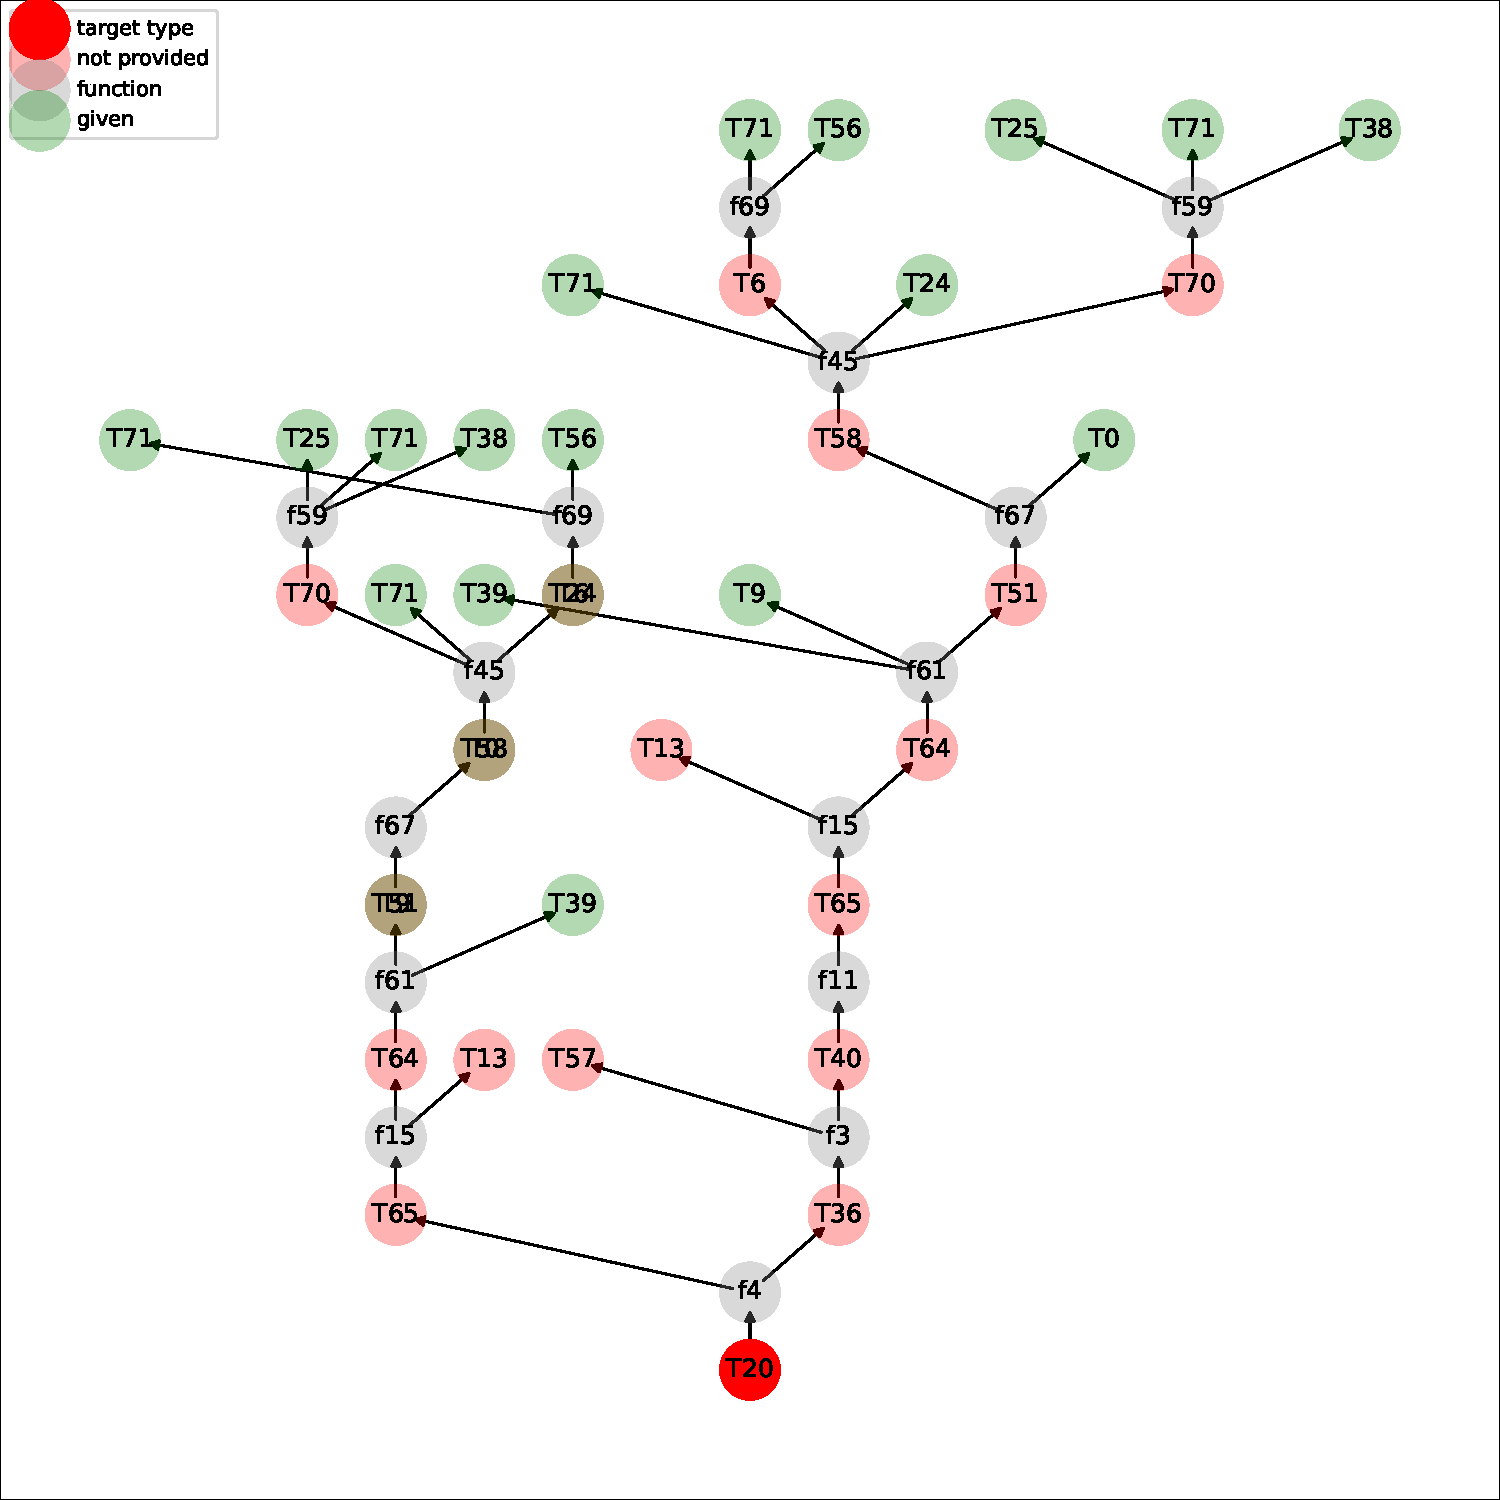
\includegraphics[width=\columnwidth]{dep_graph.pdf}
  \caption{ Dependency graph}
  The red node T35
  at the bottom represents the target that we want to
  compute: \texttt{NumericVegetationCarbonMeanBackwardTransitTimeSolution}
  The green nodes are the building blocks that we have provided in the
  model source file.
  The light red nodes show things that are not provided but have to be 
  computed via the function represented by the grey nodes. 
  This is possible if all their (ultimate recursive) dependencies
  are green nodes. 
  In this example this is the case except for nodes  T70 and T38
  \texttt{StartConditionMaker} and \texttt{VegetationCarbonStateVariableTuple} respectively 
  JAMES/TypeLegend.tex
\end{figure}  

\subsection{The biogeochemical model database \texttt{bgc\_md2}}
This is the central package and can be seen as a frontend to \CompartmentalSystems and \LAPM facilitated by \ComputabilityGraphs.
It can be used as a library \footnote{rather than a framework, since there is no `inversion of control'} 
that provides: 
  \begin{enumerate}
    \item
      Datatypes defining {\bf building blocks and comparable results} 
      specifically tailored to compartmental models.
      e.g.\ \texttt{CompartmentalMatrix}, \texttt{InternalFluxesBySymbol},
      \texttt{NumericVegetationCarbonMeanBackwardTransitTimeSolution} \dots  
      Many of these types are based on a symbolic
      mathematical representation, using \sympy, so that many symbolic results are computable 
      without the need to know parameters or data to  run the models.
      Using the underlying graph representation as sets of pools and fluxes, we can reorder pools and thereby automatically transform the compartmental matrices, group them into different subsets (e.g. vegetation, soil, litter, carbon, nitrogen \dots ), substitute pool names, get mathematical expression for cumulative fluxes e.g. from vegetation to soil or simply plot the graphs.
      Using this symbolic transformations we can compare models that might have looked very different initially, simply due to arbitrary choices of pool names or their even more arbitrary order. 
      \todo{green brown graph or link to the compare TICO notebook }
    \item
      Type annotated functions operating on those types (forming the edges of the graph where the Datatypes are nodes) 
    \item
    $30+$ vegetation, soil or ecosystem models for carbon and nitrogen cycling
      as reusable python modules using the building blocks in a flexible way. 
    \item 
      An interface to \emph{many  algorithms} in \texttt{CompartmentalSystems} to compute diagnostic variables
      for \emph{many models} in \texttt{bgc\_md2}.
  \end{enumerate}
It is impossible to fully exhibit the potential of this approach without
examples.
To this end we created some illustrative \texttt{jupyter} notebooks that are
availble via binder without the need to install the packages. 
This paragraph contains only pointers to those much more elaborate notebooks
and some example plots from them.
The examples demonstrate how \texttt{bgc_md2}:
\begin{enumerate}
\item 
  Symplifies and unifies the creation of new models from scratch while using the
  symbolic and graphic diagnostic capabilities to inspect it while we build it
  and use 
  \ComputabilityGraphs to point out what missing information we have to
  provide to make desired results computable.
  This is demonstrated in
  %\url{}
\item 
  How a model that is already part of the database can be
  inspected w.r.t complex diagnostics like the transient mean transit time that
  would take years to implement in stand alone model code but are now available
  for all models with sufficient information.
  This is demonstrated in
  %\url{}
\item 
  aided by \ComputabilityGraphs 's ability to compute which properties are computable
  allows to query the collection of models that are already part of
  \texttt{bgc\_md}.
  This is demonstrated in
  %\url{}
\item 
  Several Models for which numeric parameter values and driver data are
  available can be compared w.r.t. abstract properties.
  We chose the mean age and transit time of the vegetation and soil subsystems
  since they are defined for all models while the concrete pools of the models
  differ and not only have different names but also different meaning.
  %\url{}
\end{enumerate}

\begin{figure}[t]
	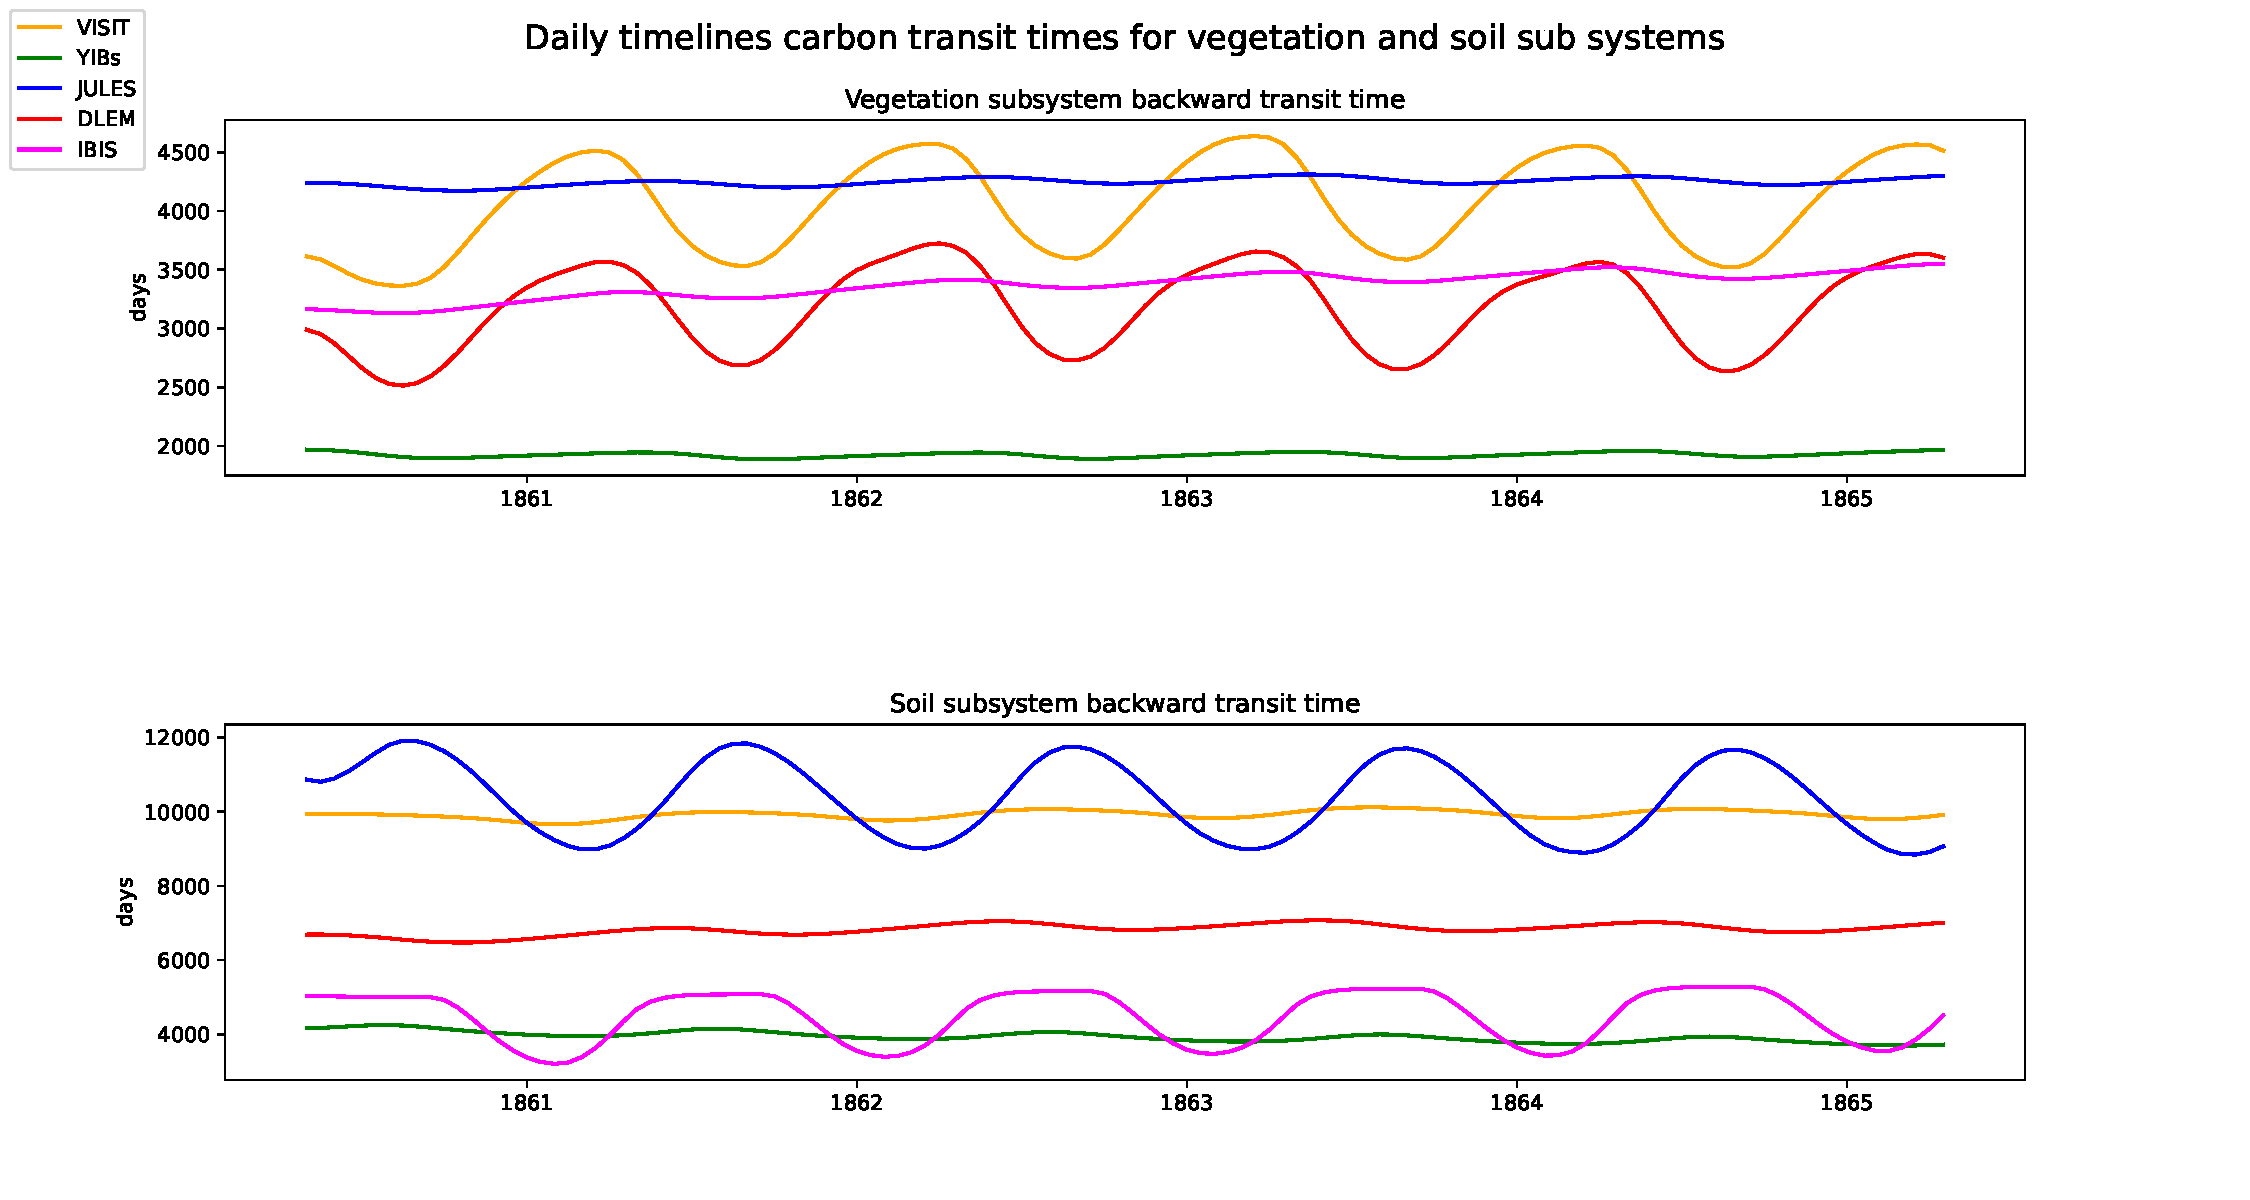
\includegraphics[width=\columnwidth]{test_veg_soil.pdf}
  \caption{
  Figure above: Comparing the (real = transient) backward transit time through 
  subsystems, accross different models. 
  }
\end{figure}  

\begin{figure}[t]
	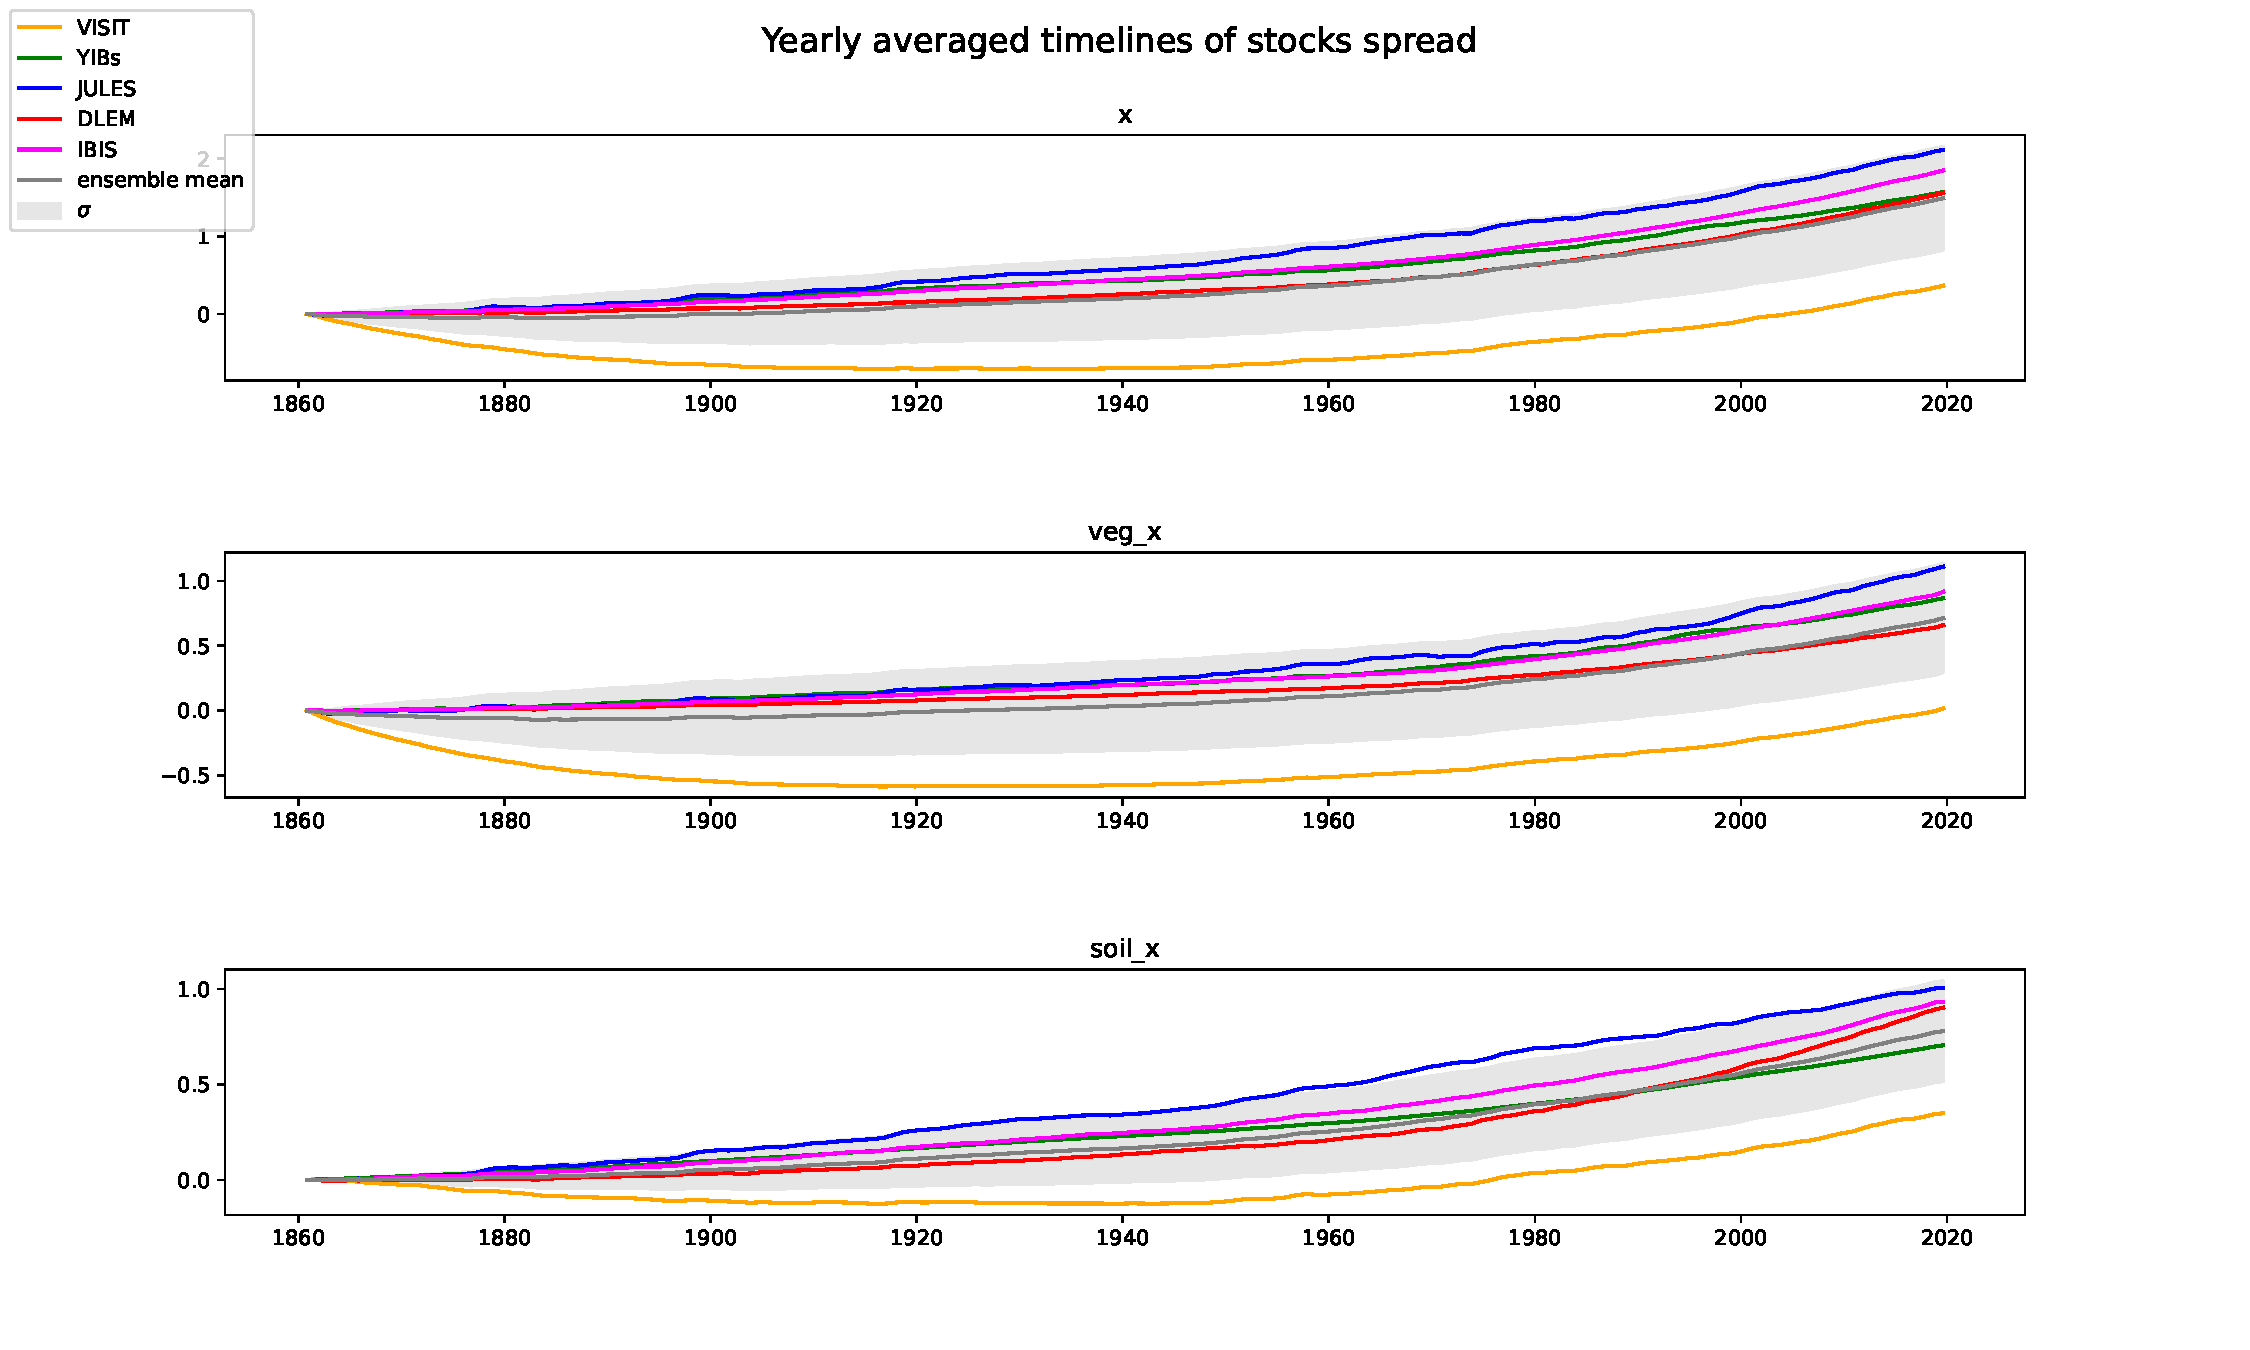
\includegraphics[width=\columnwidth]{test_stock_mean.pdf}
  \caption{
  Figure above: Total Carbon stock and subsystem stock development for different models.
  \texttt{bgc\_md} only needs to be told which pools belong to which subsystem.
  }
\end{figure}  


\begin{figure}[t]
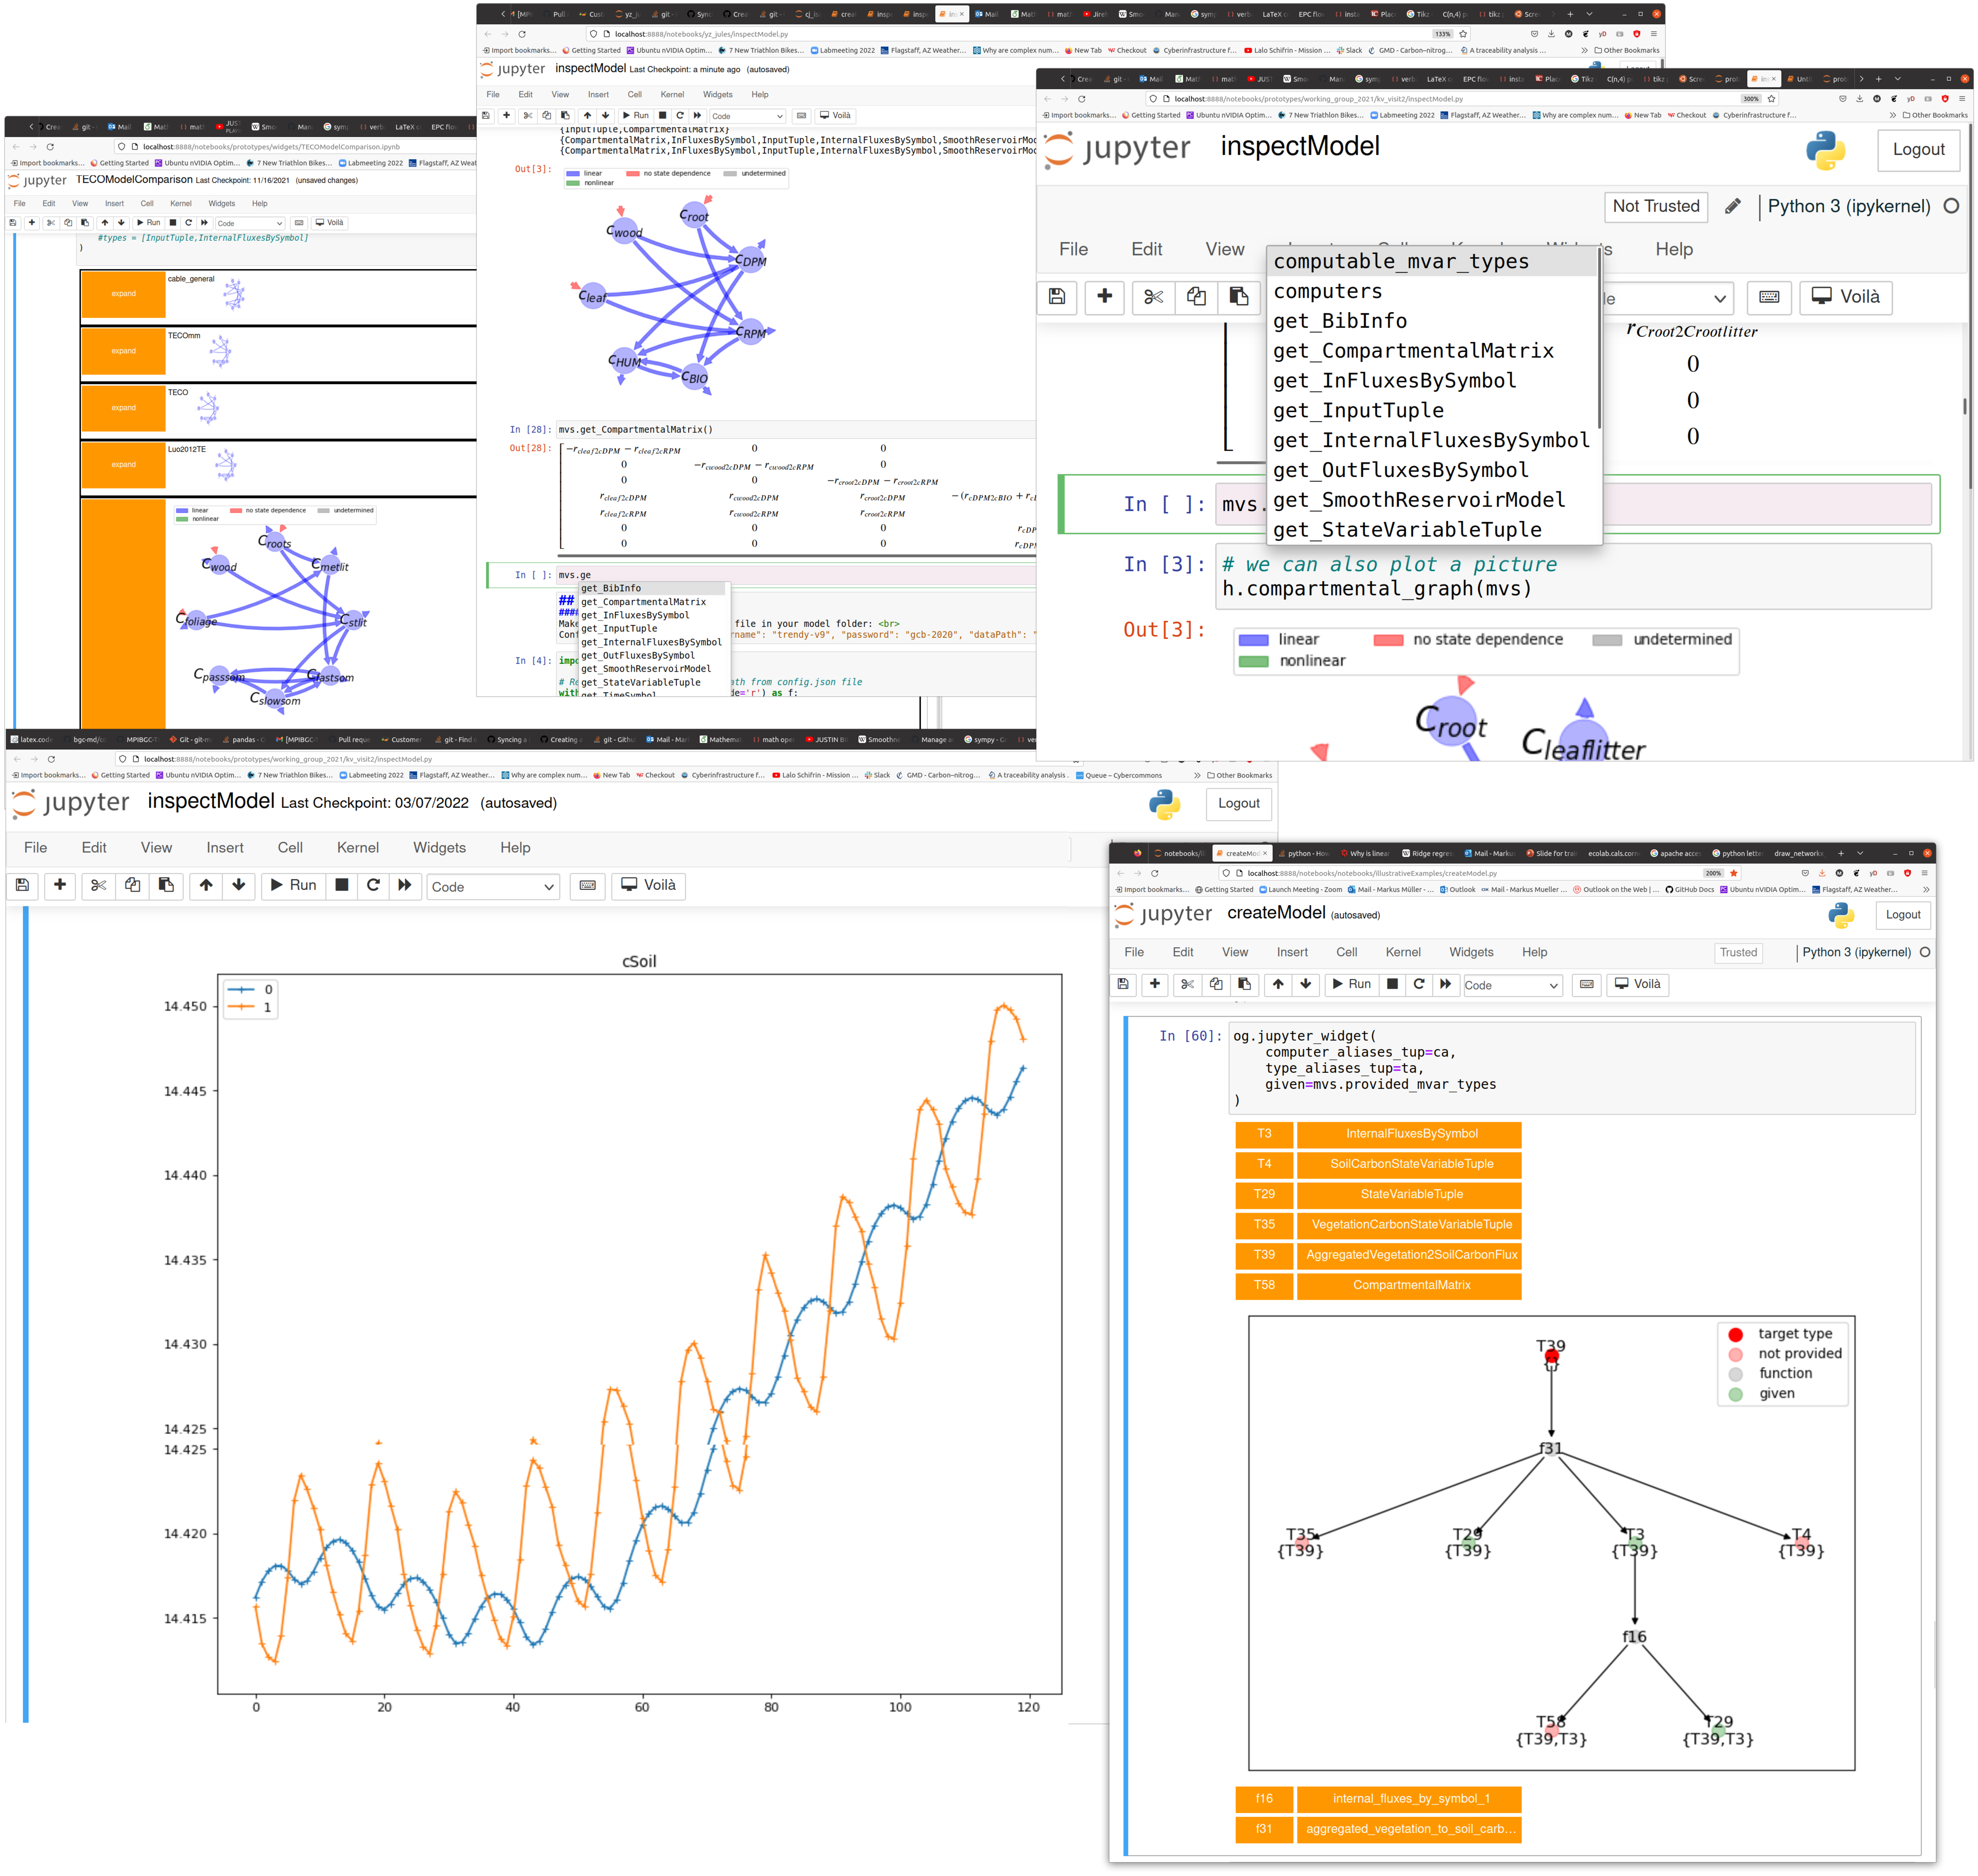
\includegraphics[width=\columnwidth]{TabScreenCombined.pdf}
  \caption{
      Figure description, top row, left to right: Interactive jupiter widget
      with a table of models (orange buttons can be clicked to expand or
      collape a more detailed view of the particular model), Model inspection
      with pool connection graph, which can be derived from the symbolic
      description along other symbolic properties as flux equations and the
      compartmental matrix, Zoom into IPython/Jupyter UI, showing methods
      automatically added by the computability graph library.  \\ Bottom row:
      Data assimilation with an automatically created numeric model (from
      symbolic description), Computability graph for a desired diagnostic
      (aggregated Flux from the vegetation to soil part, showing that the
      additionally needed information to compute the desired result)
  }
\end{figure}

%\subsection{Installation, documentation and demonstrations}
%The four packages are managed under version control in GitHub, and are publicly available for their evaluation, use, and further modification. 
%
%The four packages can be installed following the instructions provided for the
%installation of \texttt{bgc\_md2}, which depends on \LAPM and
%\CompartmentalSystems and \ComputabilityGraphs. 
%Several installation scripts exist that installs all packages at once. 
%the standard one using Conda. 
%All packages have extensive testsuites which are triggered by every commit but
%can also be run manually e.g. after installation which we strongly recommend.
%The test suites are  stored in the folder \texttt{tests} under the root of the repo . If they run successfully, then all the functionality of the four packages is readily accesible. 
%
%Detailed instructions of the installation procedure can be found in the `README.md' file of the \texttt{bgc\_md2} repository. 
%
%We use standard python docstrings to document modules, functions, classes and methods which are
%available in interactive python sessions. 
%We also compile them using Sphynx, a documentation generator for python code,
%into a hypertext documentation which is served by GitHub. It's automatically updated when changes to the documentation are pushed to the master branch of the repositories. 
%
%In addition to this documentation, we provide Jupyter notebooks for each package, with demonstrations of specific aspects of the available functionality.
%Each package has a 'notebooks' folder where the Jupyter notebooks are stored. However, they are stored as source .py files and not in the original .ipynb format. 
%The reason for this is that to maintain the notebooks under version control and avoid conflicts among different versions on different machines, we store the notebooks as regular python files. To convert these files to Jupyter notebooks, we recommend to use Jupytext, which does the translation with a simple `convert' command. 
%
%\section{Illustrative example}
%We provide an example notebook in
%https://github.com/MPIBGC-TEE/bgc_md2/tree/master/notebooks/illustrative_example.
%It shows the interplay of all four packages on the collection of predefined
%models in \texttt{bgc\_md2} and ways to extend this collection by defining a new model
%that can be compared with respect to diagnostic variables that are computed
%using \LAPM and \CompartmentalSystems.  The best way to use the example is to
%install the packages and explore the example interactively.
%\section{Impact}

\section{Conclusions}
%%% End of body of article

%%%%%%%%%%%%%%%%%%%%%%%%%%%%%%%%%%%%%%%%%%%%%%%
%% Optional Appendices go here
%
% The \appendix command resets counters and redefines section heads
%
% After typing \appendix
%
%\section{Here Is Appendix Title}
% will show
% A: Here Is Appendix Title
%
%\appendix
%\section{Here is a sample appendix}

%%%%%%%%%%%%%%%%%%%%%%%%%%%%%%%%%%%%%%%%%%%%%%%
% Optional Glossary, Notation or Acronym section goes here:
%
% Glossary is only allowed in Reviews of Geophysics
%  \begin{glossary}
%  \term{Term}
%   Term Definition here
%  \term{Term}
%   Term Definition here
%  \term{Term}
%   Term Definition here
%  \end{glossary}


%%%%%%%%%%%%%%%%%%%%%%%%%%%%%%%%%%%%%%%%%%%%%%%
% Acronyms
%% NOTE that acronyms in the final published version will be spelled out when used in figure captions.
%   \begin{acronyms}
%   \acro{Acronym}
%   Definition here
%   \acro{EMOS}
%   Ensemble model output statistics
%   \acro{ECMWF}
%   Centre for Medium-Range Weather Forecasts
%   \end{acronyms}


%%%%%%%%%%%%%%%%%%%%%%%%%%%%%%%%%%%%%%%%%%%%%%%
% Notation
%   \begin{notation}
%   \notation{$a+b$} Notation Definition here
%   \notation{$e=mc^2$}
%   Equation in German-born physicist Albert Einstein's theory of special
%  relativity that showed that the increased relativistic mass ($m$) of a
%  body comes from the energy of motion of the body—that is, its kinetic
%  energy ($E$)—divided by the speed of light squared ($c^2$).
%   \end{notation}




%%%%%%%%%%%%%%%%%%%%%%%%%%%%%%%%%%%%%%%%%%%%%%%
%
% DATA SECTION and ACKNOWLEDGMENTS
%
%%%%%%%%%%%%%%%%%%%%%%%%%%%%%%%%%%%%%%%%%%%%%%%

\section*{Open Research Section}
This section MUST contain a statement that describes where the data supporting the conclusions can be obtained. Data cannot be listed as ''Available from authors'' or stored solely in supporting information. Citations to archived data should be included in your reference list. Wiley will publish it as a separate section on the paper’s page. Examples and complete information are here:
https://www.agu.org/Publish with AGU/Publisusing SymPy'sh/Author Resources/Data for Authors
